\PassOptionsToPackage{dvipsnames}{xcolor}
\documentclass[11pt]{article}
\usepackage[titletoc,title]{appendix}

\providecommand{\datapath}{.}
\usepackage{xltxtra}
\usepackage{fontspec}
\setmainfont{Century Schoolbook}
\usepackage{placeins}
%\setmainfont{Times New Roman}
\setmathrm{Cambria Math}
\setmonofont{Consolas}
\usepackage{amssymb,amsmath}
\usepackage{datapie} 
\usepackage{nicefrac}
\usepackage{subfig}
\usepackage{filecontents} 
\usepackage{csvsimple,booktabs}
\usepackage{filecontents}
\usepackage{authblk}
\providecommand{\datapath}{.}
\usepackage{filecontents} 
\usepackage{pgfplots, pgfplotstable}
%\usepgfplotslibrary{statistics}
\usepgfplotslibrary{colormaps}
\pgfplotsset{grid style={dashed,lightgray}, compat=newest} 
\usepackage[figureposition=top,labelfont=bf]{caption}
\usepackage[newfloat]{minted}
\usepackage[textwidth=16cm,textheight=22cm]{geometry}
\usepackage[english]{babel}
\usepackage{gensymb}
\usepackage{blindtext}
\pgfplotsset{compat=newest}
\usetikzlibrary{plotmarks}
\usetikzlibrary{matrix,shapes,arrows,positioning,chains}
\usetikzlibrary{chains,fit,shapes.geometric}
\usetikzlibrary{pgfplots.units}
    \usepgfplotslibrary{units}
\usepackage{afterpage}
\usepackage[english]{babel}
\usepackage{epigraph} 
\usepackage[bottom]{footmisc}
\pretolerance=100000
\usepackage{natbib}
\widowpenalties 1 100
\usepackage{etoolbox}
\usepackage{url}
\usepackage{rotating}
\usepackage{booktabs}
\usepackage{setspace}
\usepackage{latexsym}
\usepackage{booktabs}
\linespread{1.3}
\usepackage{lipsum}
\usepackage[english]{babel}
\usepackage{upquote}
\usepackage{listings}
\usepackage{enumerate}
\usepackage{float} 
\usepackage{lscape}
\usepackage{graphicx}
\usepackage{bm}
\usepgfplotslibrary{fillbetween}
\usepackage[colorlinks = true,
            linkcolor = Mahogany,
            urlcolor  = Blue,
            citecolor = Blue,
            anchorcolor = violet]{hyperref}
\makeatletter
\makeatother
\usetikzlibrary{calc,shadings}
\newenvironment{customlegend}[1][]{%
    \begingroup
    % inits/clears the lists (which might be populated from previous
    % axes):
    \csname pgfplots@init@cleared@structures\endcsname
    \pgfplotsset{#1}%
}{%
    % draws the legend:
    \csname pgfplots@createlegend\endcsname
    \endgroup
}%
% makes \addlegendimage available (typically only available within an
% axis environment):
\def\addlegendimage{\csname pgfplots@addlegendimage\endcsname}
\pgfkeys{/pgfplots/number in legend/.style={%
        /pgfplots/legend image code/.code={%
            \node at (0.295,-0.0225){#1};
        },%
    },
}
\pgfplotsset{
   /pgfplots/bar  cycle  list/.style={/pgfplots/cycle  list={%
        {black,fill=ProcessBlue!75,mark=none},%
        {black,fill=Fuchsia!75,mark=none},%
        {black,fill=Gray!25,mark=none},%
        {black,fill=Bittersweet!75,mark=none},%
        {black,fill=NavyBlue!75,mark=none},%
        {black,fill=OliveGreen!75,mark=none},%
        {black,fill=Salmon!75,mark=none},%
			{black,fill=Yellow!75,mark=none},%
			{black,fill=WildStrawberry!75,mark=none},%
			{black,fill=YellowOrange!75,mark=none},%
       {black,fill=SeaGreen!75,mark=none},%
			}
   },
}
\pgfplotsset{
    table/myStyleWithMeta/.style={    
        meta=amount, 
    }
}

\pgfplotsset{
    discard if/.style 2 args={
        x filter/.code={
            \ifdim\thisrow{#1} pt=#2pt
                \def\pgfmathresult{inf}
            \fi
        }
    },
    discard if not/.style 2 args={
        x filter/.code={
            \ifdim\thisrow{#1} pt=#2pt
            \else
                \def\pgfmathresult{inf}
            \fi
        }
    }
}


\usepackage[many,minted]{tcolorbox}% version 3.03 or better

\newcommand{\mynewminted}[3]{%
  \newminted[#1]{#2}{#3}%
  \tcbset{myminted/#1/.style={minted language=#2,minted options={#3}}}}

\mynewminted{mycsharp}{csharp}{tabsize=2,fontsize=\small}
\mynewminted{myjson}{js}{tabsize=2,fontsize=\small}
\mynewminted{myxml}{xml}{tabsize=2,fontsize=\small}
\mynewminted{myshell}{shell-session}{tabsize=2,fontsize=\small}
\mynewminted{mycode}{text}{tabsize=2,fontsize=\small}

\newtcblisting[list inside=mypyg]{listingsbox}[3][]{%
  listing only,title={Command: \thetcbcounter: #3},
  list entry={\protect\numberline{\thetcbcounter}#3},
  enhanced,colframe=black!40,drop fuzzy shadow,myminted/#2,#1}


\tcbuselibrary{minted,skins}

\newtcblisting{bashcode}[1][]{
%  listing engine=minted,
  colback=bashcodebg,
  colframe=black!70,
  listing only,
%  minted style=colorful,
%  minted language=bash,
  minted options={linenos=true,numbersep=3mm,texcl=true,#1},
  left=5mm,enhanced,
  overlay={\begin{tcbclipinterior}\fill[black!25] (frame.south west)
            rectangle ([xshift=5mm]frame.north west);\end{tcbclipinterior}}
}
\definecolor{bashcodebg}{rgb}{1,1,1}

\renewcommand{\theFancyVerbLine}{\sffamily
\textcolor[rgb]{0.75,0.0,0}{\scriptsize
\oldstylenums{\arabic{FancyVerbLine}}}}

\captionsetup[listing]{position=top}
\SetupFloatingEnvironment{listing}{name=Code Example}
\begin{document}	
\renewcommand*{\thefootnote}{\fnsymbol{footnote}}
\title{\LARGE{An Introduction to the Command \\ Line Interface}}

\author{Charles Rahal}
\affil{Department of Sociology, University of Oxford}

\renewcommand\Authands{ and }

\footnotetext{For correspondence: Charles Rahal, Department of Sociology, University of Oxford, Manor Road Building, Manor Road, Oxford, OX1 3UQ. E-mail: \color{Blue}charlie rahal at gmail dot com\color{black}. Accompanying shell scripts for this chapter can be found at \color{Blue}github.com/crahal\color{black}, in addition to a set of slides to be delivered as a workshop.  All text in \texttt{typewriter font} indicates a command or filepath.}

\date{}
\maketitle

\begin{center}
This version: \color{Blue}\textbf{1st June, 2017}\color{black}\\ \vspace{0.15in}
This is a preliminary draft -- please send comments to \color{Mahogany}{\textbf{charlierahal@gmail.com}}
%To appear in  Mills et al. (2017): \color{Mahogany}\textbf{`An Intoduction to Sociogenomics'}  \color{black} (TBC).\\
\end{center}

\section{Introduction and History}

The command line interface (`CLI')  can often feel like a harsh, unforgiving environment, but it represents an indispensable way to interface with the underlying operating system of a computer. In comparison to graphical user interfaces (`GUI'), CLIs can require substantial effort in order to understand and acquire the skills to execute specific tasks, but conversely, they represent an almost infinite space of opportunity productive analysis which would otherwise remain largely impossible. If you are a Microsoft Windows user, you may have already encountered the command line through the `Command Prompt' (\texttt{cmd}): the counterpart of COMMAND.COM in DOS and antiquated Windows 9x systems. If you are running Mac OS X or Linux, you are already operating a `Unix-like' (hereafter `*nix-like') system with access to command line utilities (through the `terminal'), likely all neatly packaged behind an accessible graphical environment. To more concretely motivate our use of the command line in a general context, the following reasons are of specific importance:

\begin{itemize}
\item \textbf{Speed:} At the most primitive level, using a keyboard is faster than using a mouse.
\item \textbf{Automation:} No matter how complex the command or series of commands, the CLI doubles as a scripting language which can be ran as a batch, or `scheduled' to run at specific times in the future.
\item \textbf{Control:} Commands are often more powerful and precise, giving more control over the operations to be performed, and this is particularly relevant with more complex tasks.
\item \textbf{Consistency:} CLIs enable more `replicability' - either later by the original user or others, as all options and operations are invoked and documented in consistent form.
\item \textbf{Resources:} A computer which relies only on the CLI takes a lot less of the computer's system resources than a GUI.
\end{itemize}

There are additional factors which convincingly motivate bio-informaticians and social scientists to integrate the CLI into their workflow. The reduced cost of genomic sequencing -- due to the development of `Next-Generation Sequencing' (NGS) machines -- is rapidly generating enormous waves of data. Analysis of such large caches of genotype data typically requires hardware more powerful than a standard laptop or desktop computer, typically in the form of `high performance computing' (HPC). These almost exclusively run Linux or Unix, and a large volume of genomic software is only compatible with Linux or Mac OS-X based systems (such as one of the two discussed in Section \ref{genomicsoftware}). That is not to say that you should leave behind your graphical environment entirely! Some tasks are without a doubt best suited to a GUI, such as word-processing. However, tasks such as data manipulation and file management -- critical tasks in our domain -- are more naturally suited to the command line.


Before, we proceed, it might be useful to consider the history, and therefore the evolutionary distinction between Unix and other *nix-like systems. Unix was created 1969 at Bell Laboratories -- then a development division at AT\&T -- by Ken Thompson and Dennis Richie. Prior to this, all software was hardware dependent, written in assembler language. Unix was originally developed as a proprietary, commercial enterprise, with portability as a primary strength. Shortly after, researchers at the University of California, Berkley began developing Berkley Software Distribution (BSD) -- based on the AT\&T code base. This has since been rewritten to remove any copyright issues originating from the original Unix code. Commercial Unix derivatives which combined elements of Unix and BSD began appearing in the 1980s (such as AIX and Sun Solaris), but fragmentation began to cause problems. To address this issue, the Institute of Electrical and Electronics Engineers (IEEE) developed the \emph{Portable Operating System Interface for Computer Environments} (POSIX). On September 17, 1991, Linus Torvalds first released the Linux operating system kernel. It shares much of the core concepts of Unix, but, because it contains no Unix code, it can be freely shared and replicated. Specifically, the term Linux refers to the kernel, and for this reason, members of the free and open-source community strongly advocate the term GNU/Linux when referring to the operating system in order to acknowledge and promote the fact that GNU was a longstanding project begun in 1984 to develop a free operating system, with Linux merely providing the `missing piece'. This has since spun off into hundreds of `distributions', each with specific functionality. Notable examples include the Android operating system for smartphones and Chrome OS which runs on Chromebooks. Variants also appear on multiple types of embedded devices such as televisions, video games consoles and smartwatches. It is also by far the most popular server operating system in use today. Therefore, we can summarize the classification of *nix-like systems into one of the three main categories, a.) \textbf{Unix:} Commercial implementations based on the original AT\&T code, b.) \textbf{BSD:} Open source system derived from the orignial Unix and c.) \textbf{Linux:} Open source clone of Unix, written from scratch and freely distributed.

\section{An Overview of the Architecture}

At the core of every *nix-like operating system is the \textbf{kernel}, which provides a layer between the user applications and the hardware of the computer. For example, the kernel facilitates the printing of output to a command line (or visualizing graphics in a GUI) on a monitor, and writes files to the disk drive. It directs all of the actions of an operating system to work in harmony. Most *nix-like systems share a similar directory structure. The most common directories which we need to briefly itemize are listed below, with a basic summary visualization seen in Figure \ref{directorytree}:

\begin{itemize}
\item \texttt{/}: otherwise known as `root', this is the top of the file system hierarchy.
\item \texttt{/bin}: Binaries and other executable programs.
\item \texttt{/etc}: System configuration files.
\item \texttt{/home}: Home directories.
\item \texttt{/opt}: Optional/third party software.
\item \texttt{/tmp}: Temporary space, typically cleared upon every reboot.
\item \texttt{/usr}: User related programs.
\item \texttt{/var}: Variable data, such as log files.
\end{itemize}

\begin{figure}[!t]
\caption{An Example of a Simplified Directory Tree}\label{directorytree}
\centering
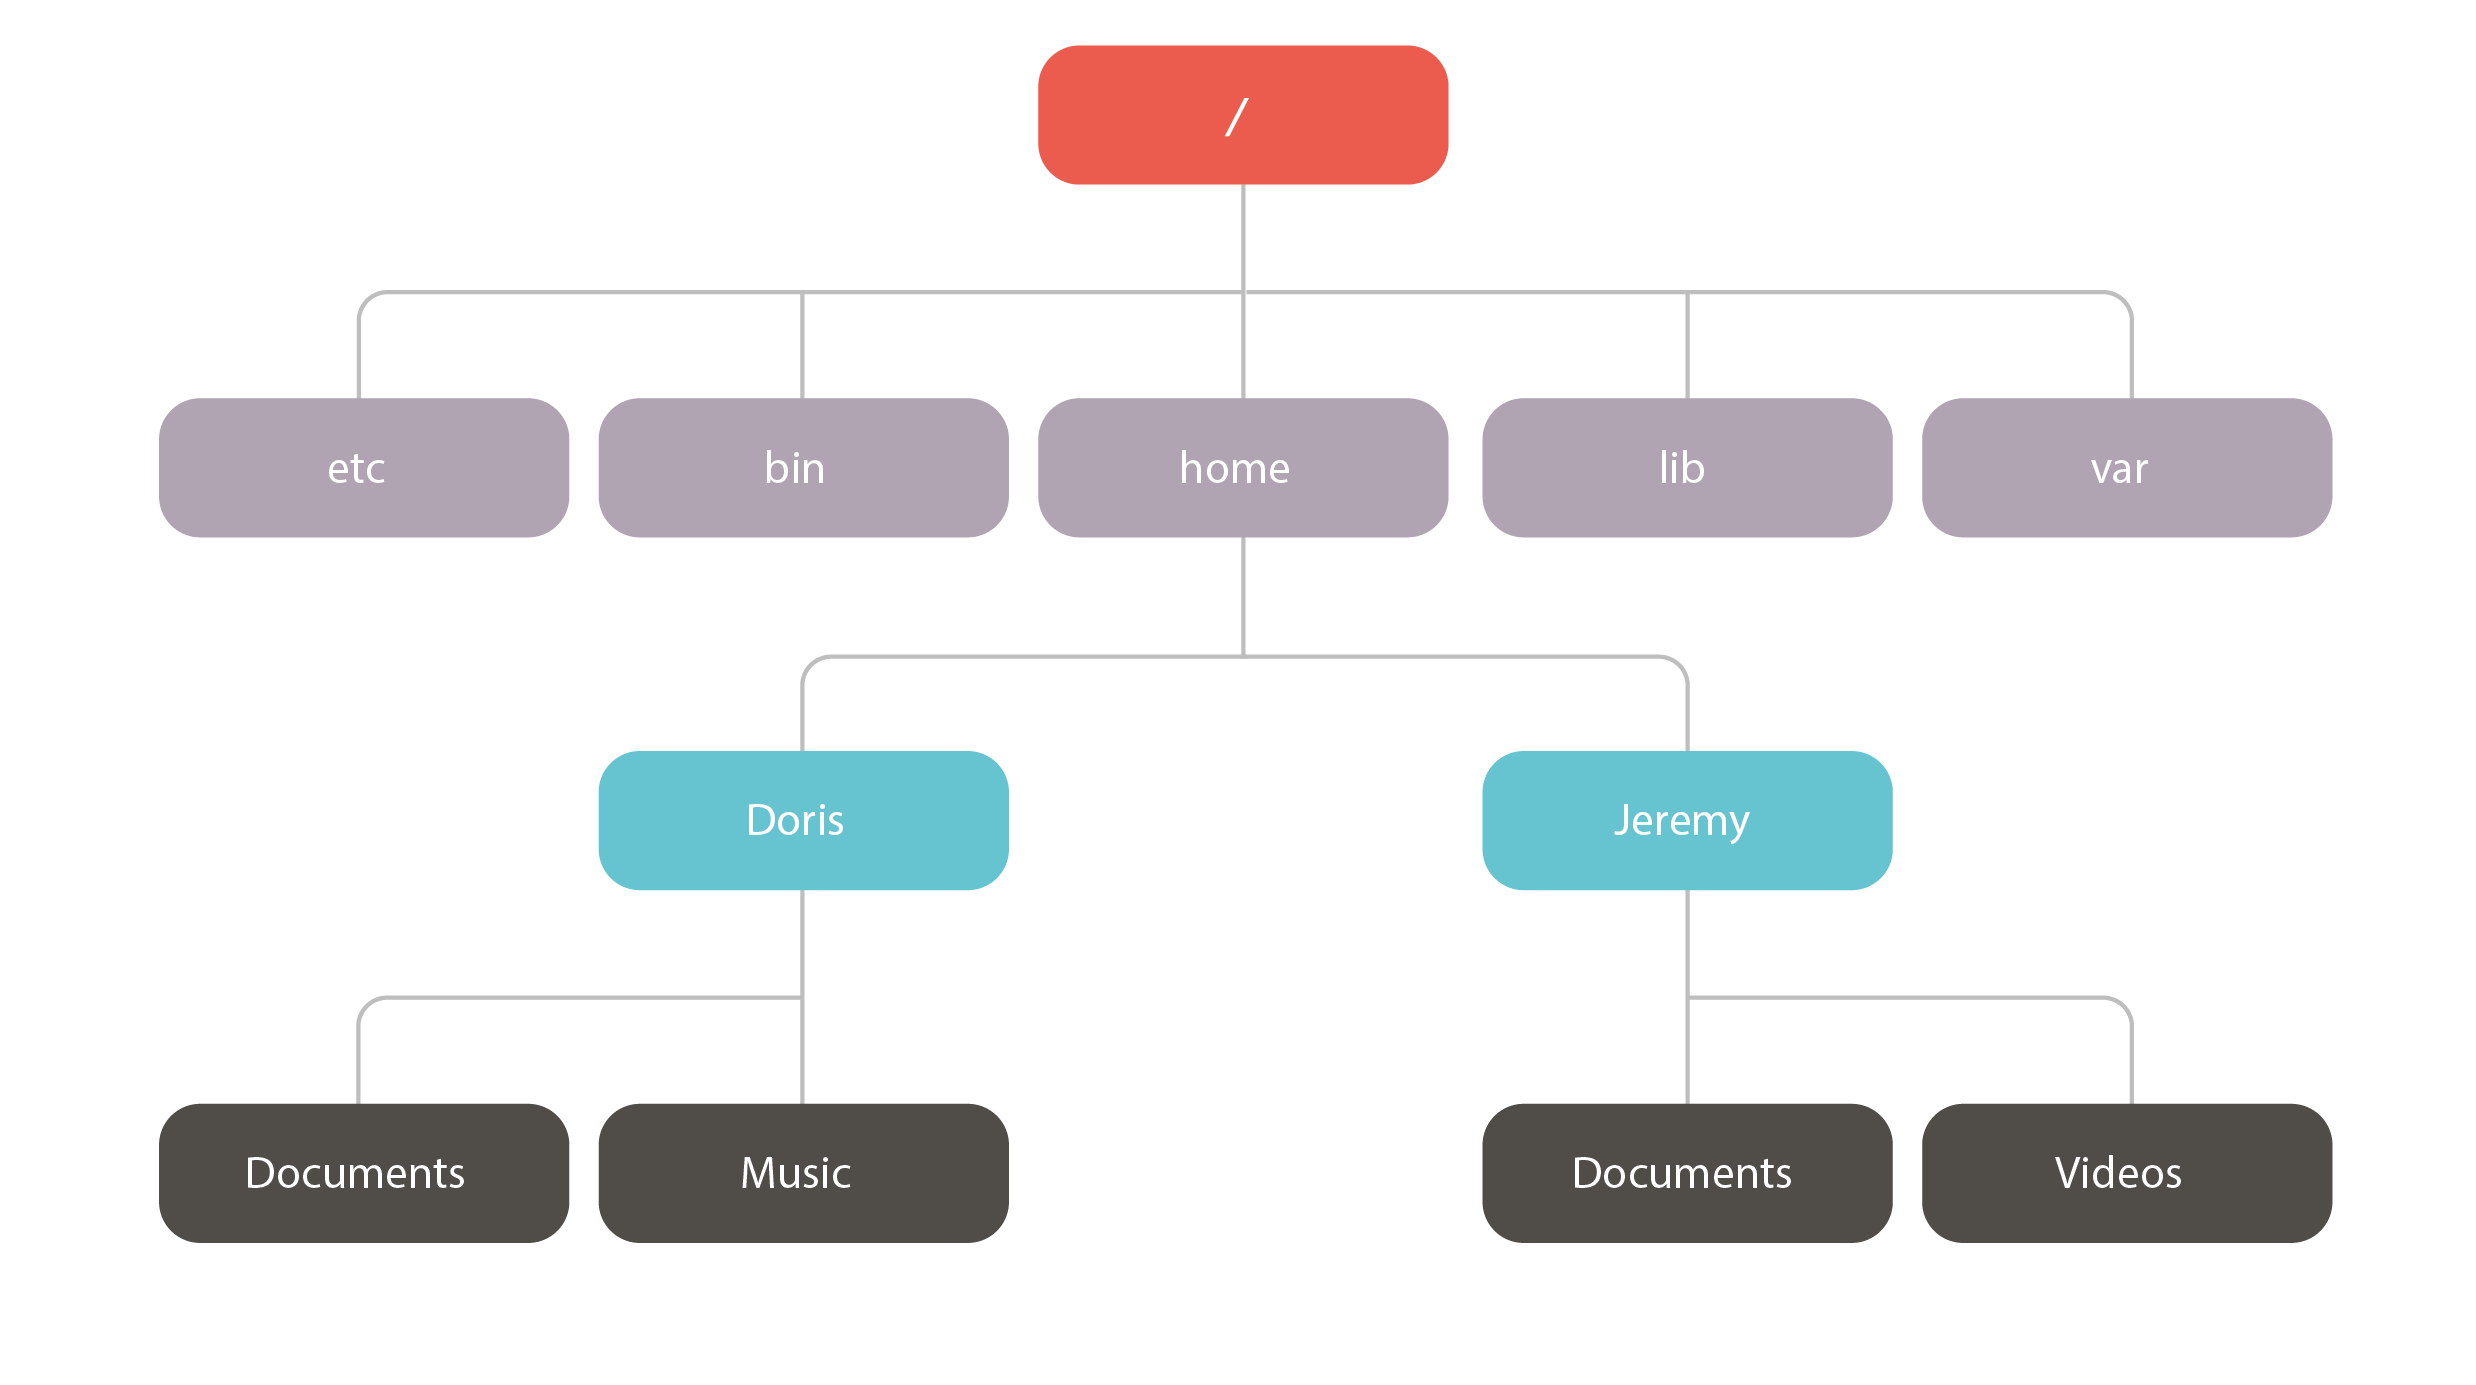
\includegraphics[width=1\textwidth]{Infographic2}
\end{figure}

User generated files are typically stored in the \texttt{/home} directory, and all files stored outside of this directory are only editable by root users. This protects core system processes either from malicious actors or accidental removal by the root user themselves. A variety of different types of file systems are supported, namely \texttt{ext2-4}, \texttt{JFS}, \texttt{HFS+}, \texttt{UFS}, \texttt{VxFS} and \texttt{ZFS}.  All have a directory known as \texttt{/dev} which contains device files pertaining to hardware installed on the system. These devices can be previewed by typing \texttt{ls -l /dev/} into the command line -- with commands and options which we will come to explain later in this chapter. 

This brings us to the \textbf{shell} -- the command line interpreter which accepts the command line inputs and performs the required tasks. At this stage, it is critical to distinguish between the two types of shell prompts: \texttt{\$} is the normal shell user, and \texttt{\#} represents the root user. These types of user have significant implications with respect to what can and cannot be accessed - where the root typically has unrestricted access (with the potential for accidental damage!). Finally, it is important to be aware that while there are many types of shells available (such as \texttt{sh}, \texttt{chs}, \texttt{tsch} and \texttt{ksh}), the Bourne Again Shell (\texttt{bash}) is by far the most popular shell in use today (where scripts for different shells are typically not portable). An overview of architecture can be seen in Figure \ref{shellandscape}.

\begin{figure}[!t]
\caption{An Overview of the Architecture}\label{shellandscape}
\centering
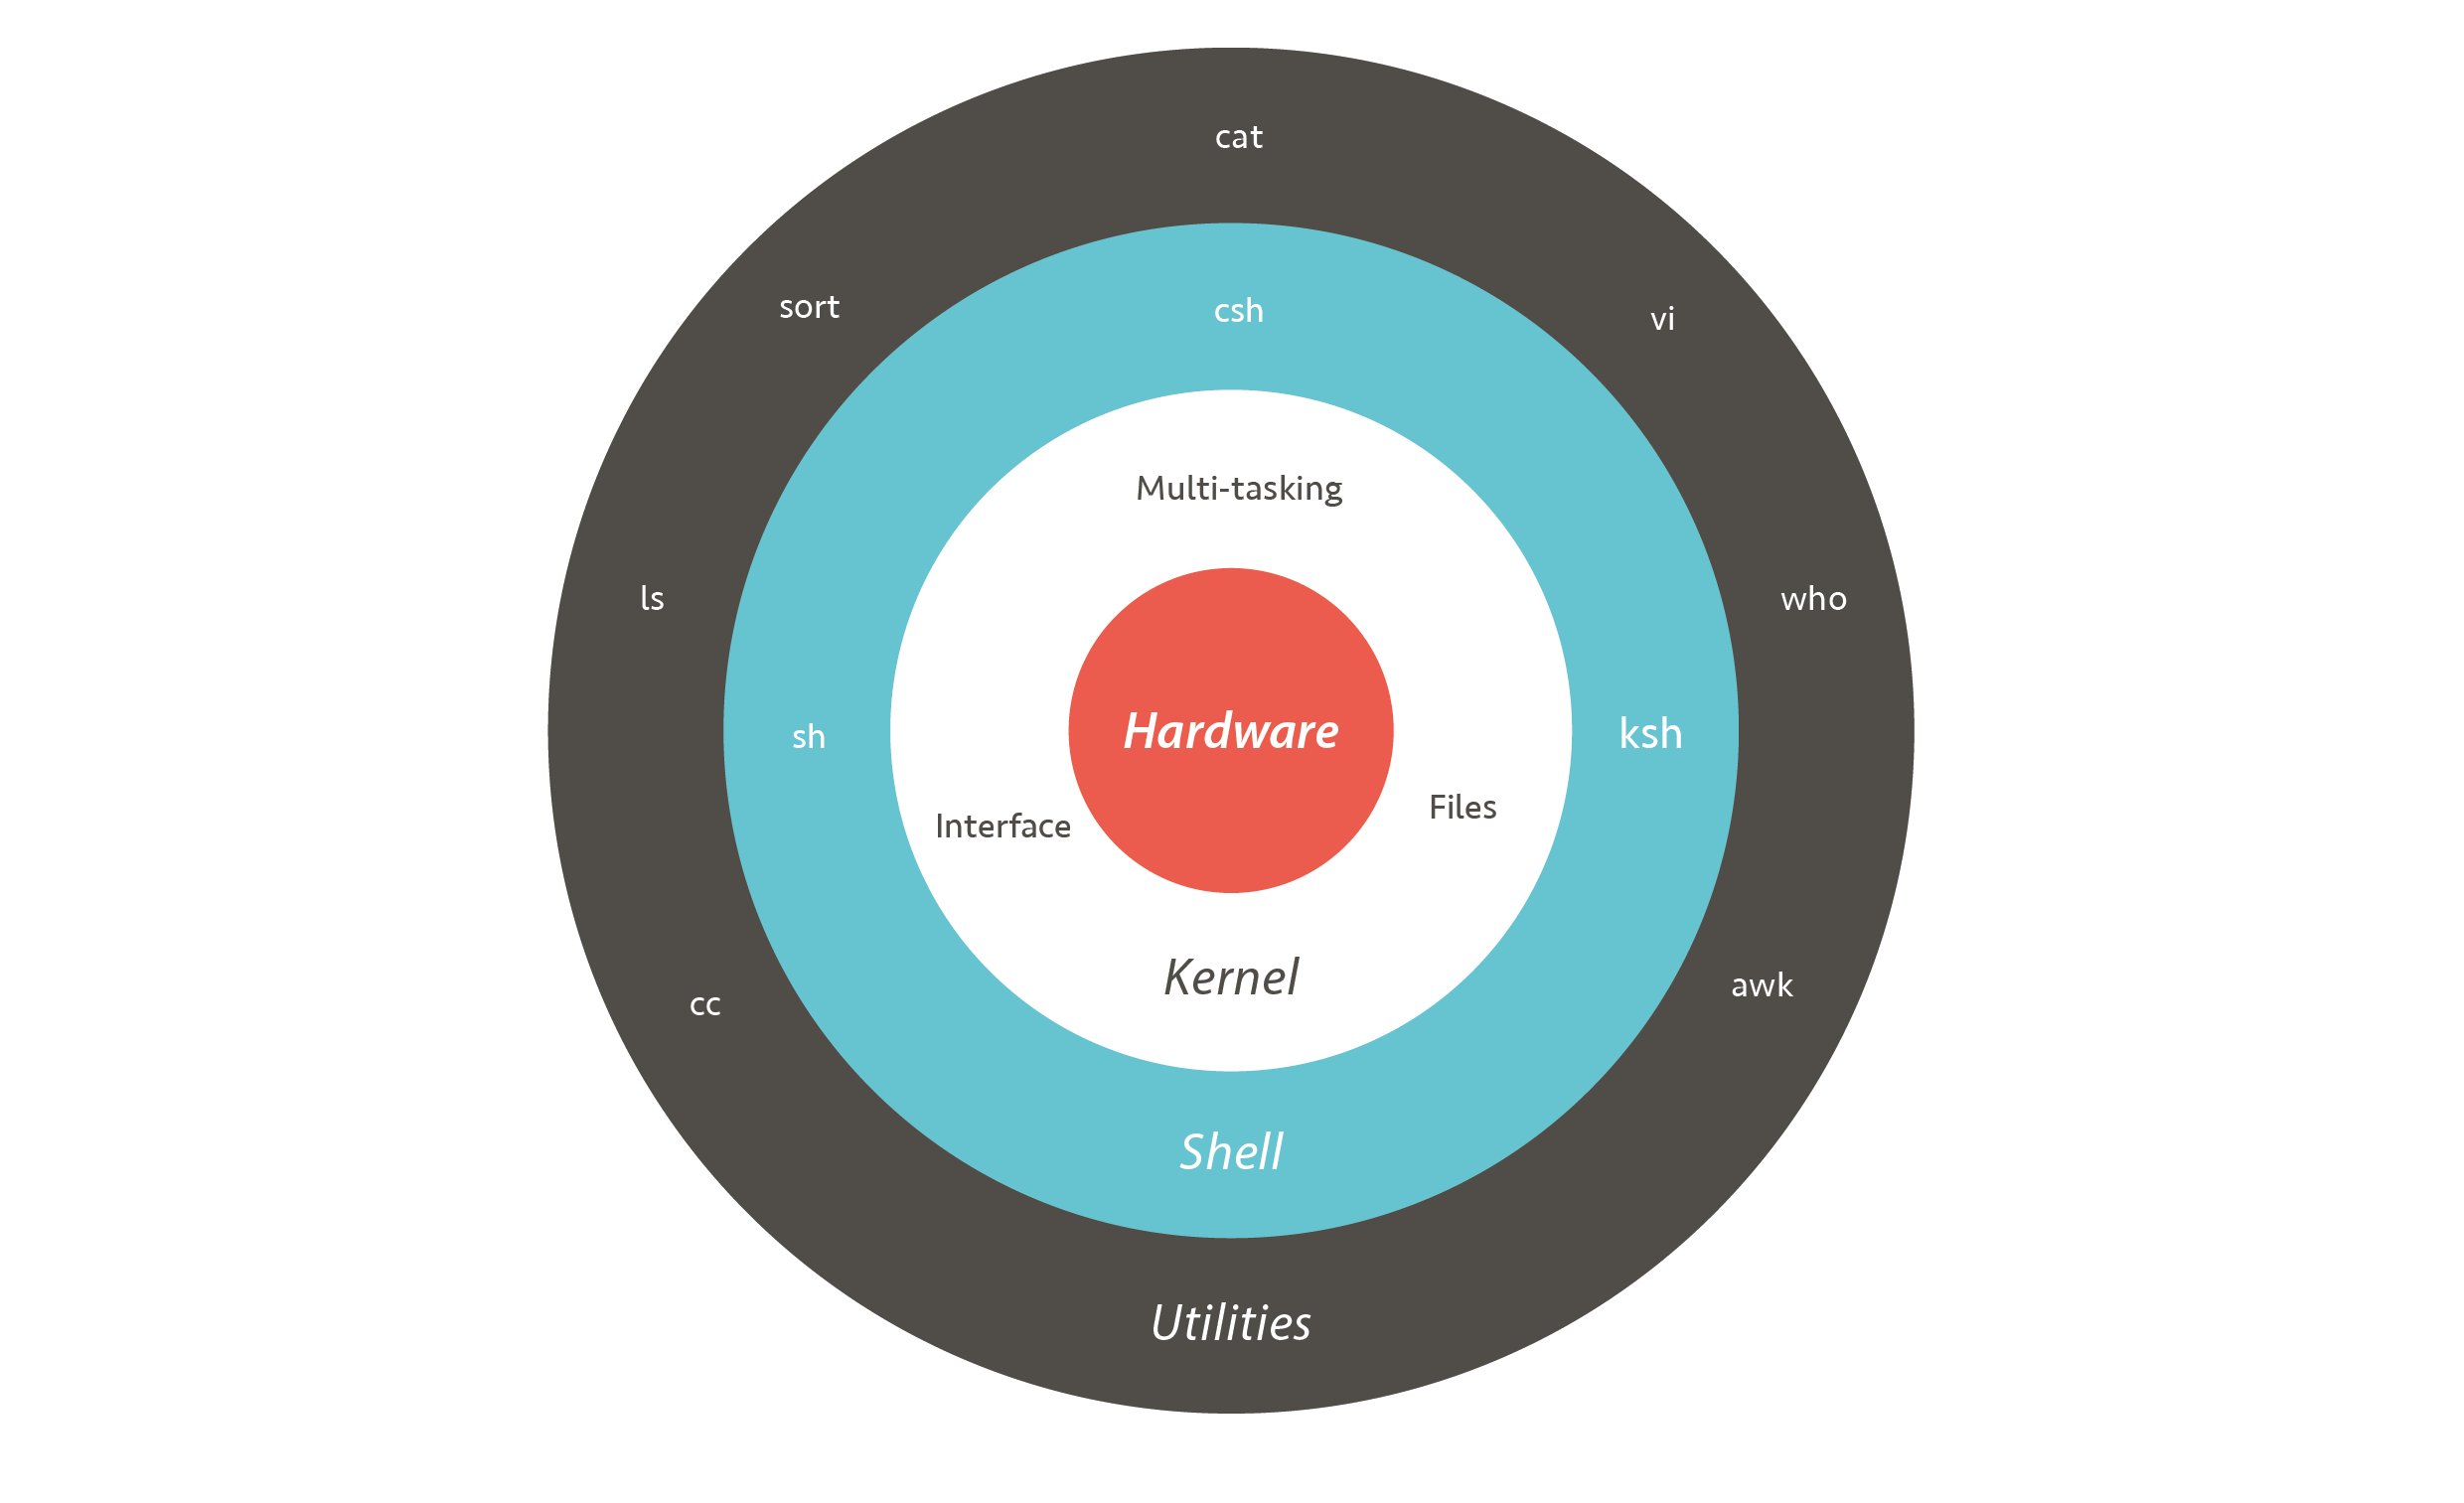
\includegraphics[width=.95\textwidth]{Infographic1}
\end{figure}

We must also mention `case sensitivity' where \texttt{ExampleFile} is \emph{not} the same as \texttt{examplefile} and the fact that there is no recycle bin (as per Windows): when you delete something from the CLI in *nix-like systems, the files are irrecoverable. One final thing to realize about *nix-like systems is that the whole philosophy revolves around a small set of building blocks and programs which we can then `pipe' together with sophisticated pattern matching and programming to create bigger things. For that reason, we start in Section \ref{fundamentalclicommands} with a set of fundamental CLI commands. Just like mathematics, learning the CLI requires practice. If you have access to a Mac or Linux, you are likely acutely aware of the value of the terminal to your system, and you can follow along without issue. If you are using Windows, one option is to create a new partition and `duel-boot' Linux alongside it, or `live-boot' from a USB directly. Another way to get access to a terminal (if you are not on a machine which natively has one) is to run Linux (or another open source Unix variant) within a virtual machine - an emulation of a computer system ran inside your default operating system. One free tool of note is VirtualBox. A final option, which may only be accessible to some readers, is to access a remote machine through their workplace or university (through the \texttt{ssh} command). Without further ado, please allow me to welcome you to the command line:\\

\begin{listing}[H]
\caption{A Warm Welcome}\vspace{-0.1in}
\begin{minted}[mathescape, linenos, numbersep=5pt, gobble=0, frame=lines, framesep=2mm]{bash}
user@system:~$ echo 'Welcome to the Command Line!'
Welcome to the Command Line!
\end{minted}
\end{listing}

\noindent
\section{Fundamental CLI Commands}\label{fundamentalclicommands}

All of the commands in the following section are summarized in the glossary at the end of this chapter. The first command which we saw in the previous section was \texttt{echo}: one of the most commonly used built-in commands which writes its arguments to standard output (the display screen by default). Another important \texttt{echo} to try is \texttt{echo \$SHELL}, which will print which shell we are using by default (where \${SHELL} is an environmental variable -- see below). The \texttt{man} command shows the manual page for a given command, including information on options and usage. This is the default resource for getting help on specific commands. For example, the \texttt{man echo} command will display the manual for the \texttt{echo} command.\\

\begin{listing}[H]
\caption{man}\vspace{-0.1in}
\begin{minted}[mathescape, linenos, numbersep=5pt, gobble=0, frame=lines, framesep=2mm]{bash}
user@system:~$ man echo
ECHO(1)                  User Commands                 ECHO(1)

NAME
       echo - display a line of text

SYNOPSIS
...
\end{minted}
\end{listing}

The \texttt{whatis} command gives a short summary description of the specific command, and command inputs can accept multiple arguments. Each manual page has a short description available within it - and \texttt{whatis} searches the manual page names and displays the manual page descriptions of any name matched. For example: \\

\begin{listing}[H]
\caption{whatis}\vspace{-0.1in}
\begin{minted}[mathescape, linenos, numbersep=5pt, gobble=0, frame=lines, framesep=2mm]{bash}
user@system:~$ whatis echo ls
echo (1)             - display a line of text
ls (1)               - list directory contents
\end{minted}
\end{listing}

\texttt{ls} is a system binary which can be accessed through the shell (with some very subtle differences to \texttt{dir}) that lists directory contents of files and directories (where different shells have different built-in commands). There are a number of important examples however. \texttt{ls /} lists the root directory. \texttt{ls ..} lists the parent directory. \texttt{ls $\sim$} lists the users home directory. The lists can also be sorted, accept wildcards, and pipe outputs to file (see below). It can show hidden files, show file size, and has the option for a `long' format.\\

\begin{listing}[H]
\caption{ls}\vspace{-0.1in}
\begin{minted}[mathescape, linenos, numbersep=5pt, gobble=0, frame=lines, framesep=2mm]{bash}
user@system:~$ ls
Desktop Documents Downloads Music Pictures Public Videos
\end{minted}
\end{listing}

However, this isn't altogether much use without knowing \emph{where} we are in the file tree. In *nix-like (and some other operating systems), the \texttt{pwd} command (which stands for print working directory) writes the full pathname of the current working directory to the standard output.\\

\begin{listing}[H]
\caption{pwd}\vspace{-0.1in}
\begin{minted}[mathescape, linenos, numbersep=5pt, gobble=0, frame=lines, framesep=2mm]{bash}
user@system:~$ pwd
/home/user
\end{minted}
\end{listing}

We can also change between the directories which we are presently in using the \texttt{cd} command (also known as \texttt{chdir}: change directory). If we carry on the example from above, we can then move from our user folder (\texttt{/home/user/}) to the Documents folder (\texttt{/home/user/Documents}). Note the change in the command prompt to indicate the change of location (on some systems):\\

\begin{listing}[H]
\caption{cd}\vspace{-0.1in}
\begin{minted}[mathescape, linenos, numbersep=5pt, gobble=0, frame=lines, framesep=2mm]{bash}
user@system:~$ cd Documents
user@system:~/Documents$ pwd
/home/user/Documents
user@system:~$ cd ..
user@system:~$ pwd
/home/user/
\end{minted}
\end{listing}

We should make a new directory (or folder - a container for other files) for the purposes of following along with these examples. This is done with the \texttt{mkdir} command:\\

\begin{listing}[H]
\caption{mkdir}\vspace{-0.1in}
\begin{minted}[mathescape, linenos, numbersep=5pt, gobble=0, frame=lines, framesep=2mm]{bash}
user@system:~$ mkdir nix
user@system:~$ ls
nix
user@system:~$ cd nix
user@system:~/nix$ pwd
/home/user/nix
\end{minted}
\end{listing}

This brings us to \emph{absolute} and \emph{relative} paths. From the documents folder above, we can navigate to the new folder (\texttt{nix}) through its relative path: \texttt{cd nix} (when we are already in \texttt{/home/user/}, or through the absolute path with \texttt{cd /home/user/nix}. There are three useful shortcuts in pathing to be aware of: $\sim$ is the shortcut for your home directory, \texttt{.} is the reference to your current directory (i.e. \texttt{cd ./nix}) and \texttt{..}, which is a reference to the parent directory. There are multiple ways of identifying the same file path in the directory tree.

The \texttt{touch} command is a standard program for Unix/Linux operating systems which is used to create, change and modify timestamps of a file.\\

\begin{listing}[H]
\caption{touch}\vspace{-0.1in}
\begin{minted}[mathescape, linenos, numbersep=5pt, gobble=0, frame=lines, framesep=2mm]{bash}
user@system:~/nix$ touch testfile
user@system:~/nix$ ls
testfile
\end{minted}
\end{listing}

Despite the lack of detail surrounding it, the file \texttt{testfile} might seem unfamiliar to you for one obvious reason: the lack of an extension. That is because we are now operating within an extensionless environment, where a file extension is normally a small set of characters after a full stop which denote which type of file it is (such as file.exe for executables, .txt for text files, and so on). In operating systems such as Windows, these are critical, as the system uses this information in order to determine how to run the file. In *nix-like systems, the extension is ignored, and the file type is determined automatically (and the command \texttt{file} can tell us additional information, if required).

Now that we've discussed how to create directories and files, we should also talk about the daunting \texttt{rm} command, which removes specified \emph{files} (by default, it does not remove directories). To remove the file we just created above, we can use the command \texttt{rm testfile}. There are two key options with the \texttt{rm} command to be aware of. \texttt{-i} (which is the short hand, where the long hand is \texttt{--interactive=always}) creates a prompt before every removal (and \texttt{-I} or \texttt{--interactive=once} creates a prompt before removing more than three files, or when removing recursively). This is the default behavior within some distributions (through bash aliases: i.e. \texttt{alias rm='rm -i'}). If the \texttt{-r} (\texttt{--recursive}) option is specified, the command will remove directories and their contents recursively. For example, we could \emph{recursively} delete the contents of the directory which we created above. \\

\begin{listing}[H]
\caption{rm}\vspace{-0.1in}
\begin{minted}[mathescape, linenos, numbersep=5pt, gobble=0, frame=lines, framesep=2mm]{bash}
user@system:~/nix$ cd ..
user@system:~/$ rm -ri nix
rm: remove directory 'nix'?
\end{minted}
\end{listing}

This not only introduces us to command \texttt{[OPTION]}s (of the form \texttt{command [OPTION]... FILE...}), but it also shows how we can stack options together, where \texttt{rm -ri} is the equivalent to \texttt{rm -r -i}. Note, that command line options are not universal between commands, and implementation across different operating systems may vary. Note how our use of \texttt{cd ..} took us up one level of the directory tree. We should also note the existence of \texttt{rmdir}, the negative equivalent to \texttt{mkdir}, which removes \emph{empty} directories. Now that we have learnt how to create files and directories, it's only natural that we learn how to move and copy them using one of the directory shortcuts we learned above (\texttt{..}).\\

\begin{listing}[H]
\caption{mv and cp}\vspace{-0.1in}
\begin{minted}[mathescape, linenos, numbersep=5pt, gobble=0, frame=lines, framesep=2mm]{bash}
user@system:~/nix$ cp testfile ..
user@system:~/nix$ rm ../testfile
user@system:~/nix$ mv testfile ..
\end{minted}
\end{listing}

An important thing to mention here is that we need not actually remove \texttt{testfile} after copying it and before moving it, as the \texttt{mv} command would simply overwrite it.

\subsection{Other Basic Utilities}

Before we move on to more advanced commands, there are a few further commands to briefly discuss. We can \texttt{clear} the terminal screen and we can also display all environmental variables with \texttt{env}. \texttt{find} and \texttt{locate} search for files and directories (with the latter being faster - performing on a database of indexed filenames after \texttt{updatedb} has been ran). \texttt{date} displays or sets (with the option \texttt{-s}) the system time, and \texttt{cal} displays the calender. \texttt{history} and specifically - \texttt{history [NUM]} reports the last \texttt{[NUM]} commands to be executed in the session. With some specific shells, the up and down arrow keys can be used to traverse the history manually. We can \texttt{exit} from the current terminal session, \texttt{logout} as a specific user, or \texttt{shutdown} the machine entirely.

\section{Slightly More Advanced Concepts}

\subsection{Editors at the Command Line}

In the last section we created files (with \texttt{touch}), but they were blank. Now is an important time to introduce the use of text editors at the command line through the use of programs such as \texttt{vi}, \texttt{pico}, \texttt{nano} and \texttt{emacs}. These programs are intended as plain text editors (as per Notepad on Windows) as opposed to a word processing suites (such as Word). They do, however, have a lot more power than Notepad (or Textedit on Mac). To use \texttt{vi} on a file, type in \texttt{vi testfile} to open a file called \texttt{testfile}. If the named file exists, then the first page of the file will be displayed in the command line, and if it doesn't, an empty file will be created (and potentially saved) and appear on the screen for editing. It is important to note, that unlike many GUI based editors, the mouse does not move the cursor. Unlike PC editors, you cannot modify text by highlighting it with a mouse. Despite these restrictions and several others, there are an extremely wide range of keyboard shortcuts which can be used to enhance productivity. Lets enter \texttt{vi} to create a file which we will use for some examples later on: a list of all the fruits we can think of (possibly with some help from \href{https://simple.wikipedia.org/wiki/List_of_fruits}{Wikipedia}). We'll save it in the \texttt{nix} directory and is call it \texttt{allfruits}.

\begin{listing}[H]
\caption{\texttt{vi allfruits}}\vspace{-0.1in}
\begin{minted}[mathescape, linenos, numbersep=5pt, gobble=0, frame=lines, framesep=2mm]{bash}
Apple
Apricot
Avocado
.
.
"allfruits" 90 lines, 846 characters
\end{minted}
\end{listing}
 
\noindent
Given the intrinsic difficulties associated with \texttt{vi} for new users (not least in \href{https://stackoverflow.blog/2017/05/23/stack-overflow-helping-one-million-developers-exit-vim/}{exiting the program}), we might recommend the use of an alternate, simpler editor (such as \texttt{nano}) where available.

\subsection{I/O Redirection}
\subsubsection{Standard Input and Output}

Now that we have a firm handle on the basic commands at our disposal, it is necessary to discuss a couple of slightly more advanced concepts before proceeding further. One of the most important facilities is the ability to redirect the input and output (`I/O') of commands, and even link commands together. As discussed above, most command line programs output their results to the `standard output' (STDOUT): which, by default, is the display. We can redirect standard output to specific files using the `>' character, and append to a file using `> >'.\\

\begin{listing}[H]
\caption{>}\vspace{-0.1in}
\begin{minted}[mathescape, linenos, numbersep=5pt, gobble=0, frame=lines, framesep=2mm]{bash}
user@system:~/nix$ ls > filelist.txt
\end{minted}
\end{listing}

While the above relates to `standard output', commands can also accept input from `standard input', (STDIN) which, by default, is the keyboard. To redirect from standard input from a file,  we use the `<' character in conjunction with the \texttt{sort} command which we will come to shortly: \\

\begin{listing}[H]
\caption{<}\vspace{-0.1in}
\begin{minted}[mathescape, linenos, numbersep=5pt, gobble=0, frame=lines, framesep=2mm]{bash}
user@system:~/nix$ sort < filelist.txt
\end{minted}
\end{listing}

There is also a third stream which will go unexamined (`standard error' or STDERR) which is used for error messages -- and also defaults to the terminal.

\subsubsection{Filters}

This brings us to a class of programs called \emph{filters}, which are extremely useful for I/O Redirection. Rather than give examples of each of them individually, we provide a list of the most commonly used filters (some of which will feature later):

\begin{itemize} 
\item \texttt{sort:} Sorts standard input then outputs the sorted result on standard output. By default it will sort alphabetically (on the first column), but there are an extremely large number of options available to modify the sorting mechanism.
\item \texttt{uniq}: Given a sorted stream of data from standard input, it removes duplicate lines of data (i.e., it makes sure that every line is unique).
\item \texttt{grep}: Examines each line of data it receives from standard input and outputs every line that contains a specified pattern of characters.
\item \texttt{fmt}: Reads text from standard input, then outputs formatted text on standard output.
\item \texttt{head}: Outputs the first few lines of its input. Useful for getting the header of a file. By default it will print the first 10 lines.
\item \texttt{tail}: Outputs the last few lines of input. Useful for things like getting the most recent entries from a log file, and is the opposite of head -- also defaults to (the last) 10 lines.
\item \texttt{cat}: Concatenates files and displays their contents, or just displays contents if given one input.
\item \texttt{cut}: Divides a file into several columns.
\item \texttt{more}: Displays output of a file one page at a time: scrolled using spacebar.
\item \texttt{less}: Displays output of a file one page at a time: scrolled up or down using arrow keys.
\end{itemize}

Two other filters to mention briefly are \texttt{nl}, which prints the line number before data, and \texttt{wc} which prints the count of lines, words and characters.

\subsubsection{The Pipe}

The final I/O redirection tool to discuss is the pipe (\texttt{|}), which allows you to connect multiple commands together. The standard output of one command is fed into the standard input of another, enabling you to chain together individual commands to create something really powerful. The example below \emph{pipes} the output from \texttt{ls} into the \texttt{head} command which takes the input \texttt{1} to show us the first 1 line of the \texttt{ls} output: we've chained the two commands together. We could optionally then redirect the standard output away from the command line into a file which contained the same output with a command such as: \texttt{ls | head -1 > myfirstpipe.txt}.\\

\begin{listing}[H]
\caption{|}\vspace{-0.1in}
\begin{minted}[mathescape, linenos, numbersep=5pt, gobble=0, frame=lines, framesep=2mm]{bash}
user@system:~/nix$ ls | head -1
allfruits
\end{minted}
\end{listing}

For even more power, it's possible to combine pipes and redirection.
\subsection{Wildcards and Regular Expressions}

Another slightly more advanced concept worth consideration is the `wildcard'.  Wildcards are a set of tools that allow you to create a pattern which defines a specific set of files or directories. There are two simple types of wildcards: 1.) \texttt{*} represents zero or more characters, 2.) \texttt{?} represents a single character. Lets create a set of files for this example called \texttt{fileonea}, \texttt{fileoneb}, \texttt{filetwoa}, \texttt{filetwob}.\\

\begin{listing}[H]
\caption{? and *}\vspace{-0.1in}
\begin{minted}[mathescape, linenos, numbersep=5pt, gobble=0, frame=lines, framesep=2mm]{bash}
user@system:~/nix$ touch fileonea fileoneb filetwoa filetwob
user@system:~/nix$ ls file*a
fileonea filetwoa
user@system:~/nix$ ls filetwo?
filetwoa filetwob
\end{minted}
\end{listing}

A regular expression (or `regex') includes such functionality, but is a much more powerful pattern matcher providing the ability to restrict the specific type of characters which are searched for. This allows a more flexible specification overall. There are a number of books dedicated exclusively to regular expressions, and a detailed examination of the subject is far beyond the scope our endeavor. Below we can list a small number of regular expression operators and then provide two quick examples to combine this functionality with the powerful \texttt{grep} command which wasn't fully explored above.

\begin{itemize}
\item \texttt{.} : Match any character.
\item \texttt{\^{}} : Match the empty string at the beginning of a line or string.
\item \texttt{\$} : Match the empty string at the end of a line.
\item \texttt{A} : Match an uppercase i.e. A.
\item \texttt{a} : Match a lowercase a.
\item \texttt{$\backslash$d} : Match any single digit.
\item \texttt{$\backslash$D} : Match any single non-digit character.
\item \texttt{$\backslash$w} : Match any single alphanumeric character.
\item \texttt{[A-E]} : Match any of uppercase A, B, C, D, or E (most commonly seen as [A-Z]).
\item \texttt{[\^{}A-E]} : Match any character except uppercase A, B, C, D, or E.
\item \texttt{(abc|xyz)} : Match a sequence of at least one of abc or xyz. 
\end{itemize}

Remember from above: the \texttt{grep} utility filters input, looking for matches. In the simplest use, \texttt{grep} prints those lines that contain text that matches a pattern. In our example, we pass it the -E option, which allows it to interpret the pattern as an extended regular expression.\\

\begin{listing}[H]
\caption{grep -E}\vspace{-0.1in}
\begin{minted}[mathescape, linenos, numbersep=5pt, gobble=0, frame=lines, framesep=2mm]{bash}
user@system:~/Documents$ grep -E [z] allfruits
Yuzu
user@system:~/Documents$ grep -E ^'(Red|Blue)' allfruits
Blueberry
Redcurrent
\end{minted}
\end{listing}

The first example searches for any fruit which contains the lowercase character z (\texttt{[z]})  in the list of fruits, where the only fruit meeting this criteria is the yuzu - a citrus fruit which looks like a small grapefruit originating from China and Tibet. The second \texttt{grep} command looks for instances at the start of the line (\texttt{\^}{ } ) which contain either `Red' or `Blue'.  Further to these tools, \texttt{awk} is another powerful utility for text processing and pattern matching which can be used to perform batch processing functions (such as renaming multiple files). However, covering it fully is far beyond the scope of this chapter.
\subsection{Users, Groups and Permissions}

Permissions  specify what a user can and cannot do - perhaps, for example, you want to lock your files in such a way that other people cannot change them, or perhaps you want to secure system files from damage. Permissions are split into three distinct categories which govern the ability to read (\texttt{r}), write (\texttt{w}) and execute (\texttt{x} - reserved for programs, scripts and directories). For every file, we need to define each of these permissions for three sets of potential users: the owner of the file, the group which owns the file, and everyone else. There are typically only two people who can manage the permissions of a given file or directory: the owner and the root user. Groups are used to simplify the management of system security, where users can be a member of one or more groups (and at least one by default). To view the permissions associated with an individual file, we can use the \texttt{-l} option on the \texttt{ls} command:\\

\begin{listing}[H]
\caption{ls -l}\vspace{-0.1in}
\begin{minted}[mathescape, linenos, numbersep=5pt, gobble=0, frame=lines, framesep=2mm]{bash}
user@system:~/nix$ ls -l allfruits
-rw-rw-r-- 1 user user 846 May 29 14:57 allfruits
\end{minted}
\end{listing}

How can we interpret this? The first character to the left determines whether it is a file (\texttt{-}), a directory (\texttt{d}) or something less common (such as a link: \texttt{l}).  Following this, we have information on the permissions for the owner, where \texttt{r}, \texttt{w} and \texttt{x} are described as above. If the permissions are missing, a \texttt{-} represents the omission of a permission. For example, with regards to \texttt{allfruits} as above, the owner of the file has read and write but not execute permissions. The same is true for the group of the owner, but everyone else only has read permission. To change the permissions associated with a file or a directory, we need to use the \texttt{chmod} command, where, again, the permission arguments are made up of three components: 1.) Who are we changing the permission for? The user (\texttt{u}), others (\texttt{o}), the group (\texttt{g}), or all (\texttt{a})? 2.) Are we giving (\texttt{+}) or taking permission away (\texttt{-})?, 3.) Which of the three permissions are we setting - \texttt{r}, \texttt{w} or \texttt{x}? Lets look at an example whereby we remove the read permissions from the group of the owner and others:\\

\begin{listing}[H]
\caption{chmod}\vspace{-0.1in}
\begin{minted}[mathescape, linenos, numbersep=5pt, gobble=0, frame=lines, framesep=2mm]{bash}
user@system:~/nix$ chmod og-r allfruits
user@system:~/nix$ ls -l allfruits
-rw------- 1 user user 846 May 29 15:09 allfruits
\end{minted}
\end{listing}

There is also a `shorthand' method which can achieve the same objectives (e.g. \texttt{chmod 751 allfruits}). There exists the same series of permissions for directories, albeit with slightly different meanings.  In the directory context (\texttt{d}), \texttt{r} means you have the ability to read what's in the directory, \texttt{w} gives the permission to write new files and directories into it, and \texttt{x} gives you the permission to enter into it. Importantly,  permissions are not inherited from the parent directory - and the recursive option (\texttt{-R}) for \texttt{chmod} can be especially useful. Other important commands include  \texttt{chown} which changes the owner of a file or directory, and \texttt{chgrp} which changes the group associated with a file or directory. The \texttt{groups} command prints which groups a user is in.

\subsection{Archiving}

Archiving in our context is equivalent to the \texttt{.zip} extension in Windows. The standard way to do this is to use the \emph{tape archive} -- \texttt{tar}. It creates and manipulates archive files -- extracting from \emph{tar}, \emph{pax}, \emph{jar}, etc, with the \texttt{-x} option, and creating them with the \texttt{-c} option. One reason why you might want to use tape archives is if you want to transfer files, but if this is your motivation, you usually want to compress the files also. The typical *nix ways to compress archives are to either use \texttt{gzip} (Lempel-Ziv coding) or \texttt{bzip2} (Burrows-Wheeler block sorting) compression. Lets see some simple examples, first making a second file from our \texttt{allfruits} list to \texttt{tar} them together before zipping them.\\

\begin{listing}[H]
\caption{tar, gzip and bzip2}\vspace{-0.1in}
\begin{minted}[mathescape, linenos, numbersep=5pt, gobble=0, frame=lines, framesep=2mm]{bash}
user@system:~/nix$ head -5 allfruits > top5fruits
user@system:~/nix$ ls -l
-rw------- 1 user user  846 May 30 13:32 allfruits
-rw-rw-r-- 1 user user   38 May 30 13:33 first5fruits
user@system:~/nix$ tar -cvf fruits.tar allfruits first5fruits
user@system:~/nix$ gzip fruits.tar
user@system:~/nix$ tar -cvf fruits.tar allfruits first5fruits
user@system:~/nix$ bzip2 fruits.tar
user@system:~nix$ bzip2 ls -l
-rw------- 1 user user 10240 May 30 14:07 allfruits
-rw-rw-r-- 1 user user    38 May 30 13:33 first5fruits
-rw-rw-r-- 1 user user   214 May 30 14:13 fruitlists.tar.bz2
-rw-rw-r-- 1 user user   224 May 30 14:13 fruitlists.tar.gz
\end{minted}
\end{listing}

\noindent
We more commonly create the archive and compression in one step with options like \texttt{-cz}, \texttt{-xz} (for gzip) and \texttt{-cj}, \texttt{-xj} for (bzip2).

\section{Bash Scripting}

Bash scripting represents a powerful tool which allows you to perform complex, and often repetitive tasks with minimal effort. We are essentially writing a series of commands (as above) which tell the Bash shell what to do next. A bash script is nothing more than a plain text file which contains commands which could also be taken out be ran on the command line. While not necessary, a extension of \texttt{.sh} helps others identify the files as shell scripts. Lets create our first script (called \texttt{myfirstscript.sh} and describe how it works:\\

\begin{listing}[H]
\begin{minted}[mathescape, linenos, numbersep=5pt, gobble=0, frame=lines, framesep=2mm]{bash}
#!/bin/bash
echo Hello There! Welcome to Bash Scripting!
\end{minted}
\end{listing}

The first line is called the `shebang'. When a script with a shebang is ran, the program loader parses the rest of the script's initial line (after \#!) as an interpreter directive - the path to the program that should be used to run the rest of the lines in the text file. The second line is the \texttt{echo} command which we saw above, and prints the message to the STDOUT. We can execute the script in two ways to obtain the same result (although there are differences between the two methods):\\

\begin{listing}[H]
\caption{./ and bash}\vspace{-0.1in}
\begin{minted}[mathescape, linenos, numbersep=5pt, gobble=0, frame=lines, framesep=2mm]{bash}
user@system:~/nix$ ./myfirstscript.sh
Hello There! Welcome to Bash Scripting!
user@system:~/nix$ bash myfirstscript.sh
Hello There! Welcome to Bash Scripting!
\end{minted}
\end{listing}

It is important to check the file permissions (especially: \texttt{x} for the first method) before trying to execute a \texttt{.sh} script. Now that we've learned to execute the scripts, we can begin to learn about variables: temporary methods of storing information. There are two key actions: setting - which requires no \$, and reading, which does. Lets see an example of how we can pass a variable to the script (called \texttt{variables.sh}), by defining a simple echo script as above which accepts \$1 and \$2 as inputs:\\

\begin{listing}[H]
\begin{minted}[mathescape, linenos, numbersep=5pt, gobble=0, frame=lines, framesep=2mm]{bash}
#!/bin/bash
echo Hello $1! Message sent from $2!
\end{minted}
\end{listing}

We can then execute it as before:\\

\begin{listing}[H]
\caption{variables}\vspace{-0.1in}
\begin{minted}[mathescape, linenos, numbersep=5pt, gobble=0, frame=lines, framesep=2mm]{bash}
user@system:~/nix$ ./variables.sh Reader Author
Hello Reader! Message sent from Author!
\end{minted}
\end{listing}

There are also a number of special variables which we need to mention:
\begin{itemize}
\item \texttt{\$0} : The filename of the current script.
\item \texttt{n} :  The arguments with which a script was invoked.
\item \texttt{\$\#} : The number of arguments supplied.
\item \texttt{\$?} : The exit status of the last command.
\item \texttt{\$\$} : Process number of the current shell.
\end{itemize}

We can also set our own variables such as \texttt{ourvariable=value}. Remembering this, and the fact that if  we want variables with more complex values however we need quotations, lets try a second example (called \texttt{settingvariables.sh}):\\

\begin{listing}[H]
\begin{minted}[mathescape, linenos, numbersep=5pt, gobble=0, frame=lines, framesep=2mm]{bash}
#!/bin/bash
recipient='Person One'
sender='Person Two'
echo Hello $recipient. Sent from: $sender
\end{minted}
\end{listing}

\noindent
Which is then executed to give:\\

\begin{listing}[H]
\caption{setting variables}\vspace{-0.1in}
\begin{minted}[mathescape, linenos, numbersep=5pt, gobble=0, frame=lines, framesep=2mm]{bash}
user@system:~/nix$ ./settingvariables.sh
Hello Person One! Message sent from Person Two!
\end{minted}
\end{listing}
We can also substitute the output of a command or program and save it to the value of a variable and export it elsewhere. We can also design shell scripts (\texttt{readvariable.sh})to ask the user for input using the \texttt{read} command. For example:\\

\begin{listing}[H]
\begin{minted}[mathescape, linenos, numbersep=5pt, gobble=0, frame=lines, framesep=2mm]{bash}
#!/bin/bash
echo Hey, Buddy! What is your favorite color?
read favoritecolor
echo Wow! $favoritecolor is my favorite color too!
\end{minted}
\end{listing}

And then execute it as:\\

\begin{listing}[H]
\caption{bash reading variables}\vspace{-0.1in}
\begin{minted}[mathescape, linenos, numbersep=5pt, gobble=0, frame=lines, framesep=2mm]{bash}
user@system:~/nix$ ./readvariable.sh
Hey, Buddy! What is your favorite color?
Blue
Wow! Blue is my favorite color too!
\end{minted}
\end{listing}

We can also do simple arithmetic operations using the \texttt{let} and \texttt{expr} commands. We can utilize the standard operators of \textbf{+}, \textbf{-}, \textbf{$\backslash$*},\textbf{ /} which represent add, subtract, multiple and divide, as well as \textbf{var++} for `increase by one' and \textbf{var--} for `decrease by one'. Finally, we can calculate the modulus with \%. In particular, \texttt{let} stores the variable, but \texttt{expr} prints it out. Lets try out each of these features, feeding variables into our script: \\

\begin{listing}[H]
\begin{minted}[mathescape, linenos, numbersep=5pt, gobble=0, frame=lines, framesep=2mm]{bash}
#!/bin/bash
let "a = $1 + $2"
echo adding $1 and $2 together gives $a
echo multiplying $1 and $2 together gives $(expr $1 \* $2)
\end{minted}
\end{listing}

\noindent
And then execute it as:\\

\begin{listing}[H]
\caption{bash arithmetic}\vspace{-0.1in}
\begin{minted}[mathescape, linenos, numbersep=5pt, gobble=0, frame=lines, framesep=2mm]{bash}
user@system:~/nix$ ./arithmetic.sh 10 5
adding 10 and 5 together gives 15
multiplying 10 and 5 together gives 50
\end{minted}
\end{listing}
\noindent
We can also embed if statements, just like in other languages:\\

\noindent
\texttt{if [ condition ]\\
then\\
\quad< execute commands >\\
fi}\\

\noindent with everything between \texttt{if} and \texttt{fi} being executed. There is no need to indent, and we can also further augment the script with nested statements, \texttt{else}, \texttt{elif}; and so on. We can also utilize various types of loops; \texttt{while}, \texttt{until} and \texttt{for} which we can \texttt{continue} and \texttt{break} out of as expected. We can also define custom functions, although this is a more advanced topic to be left for another discussion.


\section{Sociogenomics Specifics}

Now that we have a fuller understanding of the command line, we move on to some specific examples related to genomics. In particular, we'll outline three practical applications: some basic commands used on genomics data, executing scripts in languages most useful for sociogenomics (R and Python), and then executing genomics related programs to undertake a common task (calculating polygenic scores).

\subsection{Apples}

We're first going to take genome and annotations files related to apples (\texttt{apple.genome} and \texttt{apple.gene}) in order to answer a list of practical questions. The genome file is a Multi-FASTA format, as shown below:\\

\begin{listing}[H]
\caption{more apple.genome}\vspace{-0.1in}
\begin{minted}[mathescape, linenos, numbersep=5pt, gobble=0, frame=lines, framesep=2mm]{bash}
user@system:~/nix$ more apple.genome
>chr1
ATTTTTTTTCCTTTTGTTTTTGCATACAAGTCAATTTCATTCGAA
GTTTGGTTGGATCGAAAAGTCGGGGTTCAATTTTTTGATCCGAC
CACAATCAAGCTTCAACCTATGAAGATTGTCAATTTGGCCAAGG
AAAGAGTTAGGCGACCTGTTTTGACATTTGAAAAGGAAATATG
GTTGGCCTGGAAGAAAATATTCAAGTTTCTATGCCA AATATAAA
AATTGATTCAGAAGGTGATTCGTCGAATAAATGCTTAGATGATGA
...
\end{minted}
\end{listing}

Using the commands which we learned above, we can calculate the number of chromosomes in the genome using the fact that each chromosome begins with a header line which includes the distinctive character `>' (and this could be extended to \texttt{\^{}>} to ensure that it only matches where it is the first character). Therefore, we can use a combination of \texttt{grep}, \texttt{|} and \texttt{wc} to calculate the number of chromosomes:\\

\begin{listing}[H]
\caption{grep apple.genome}\vspace{-0.1in}
\begin{minted}[mathescape, linenos, numbersep=5pt, gobble=0, frame=lines, framesep=2mm]{bash}
user@system:~/nix/$ grep '>' apple.genome | wc -l. 
3
\end{minted}
\end{listing}

We can also answer a series of descriptive questions based on the \texttt{apple.genes} file. These include things like `How many genes are there?', `How many transcript variants are there?' and `How many genes have a single splice variant?'. As always, we can first have a glance at the file to check that it is the format which we expect: \\

\begin{listing}[H]
\caption{head apple.genes}\vspace{-0.1in}
\begin{minted}[mathescape, linenos, numbersep=5pt, gobble=0, frame=lines, framesep=2mm]{bash}
user@system:~/nix$ head -3 apple.genes
MDP0000303933    MDP0000303933    chr1    -    4276    5447    ...
MDP0000223353    MDP0000223353    chr1    +    77339    79628    ...
MDP0000322928    MDP0000322928    chr1    +    103533    103686    ...
\end{minted}
\end{listing}

\noindent
And then undertake the analysis: \\

\begin{listing}[H]
\caption{grep and cut apple.genes}\vspace{-0.1in}
\begin{minted}[mathescape, linenos, numbersep=5pt, gobble=0, frame=lines, framesep=2mm]{bash}
user@system:~/nix$ cut -f1 apple.genes | sort -u | wc -l
5453 
user@system:~/nix$ cut -f2 apple.genes | sort -u | wc -l
5456 
user@system:~/nix$ cut -f1 apple.genes | uniq -c | grep ' 1 ' | wc -l
5450
\end{minted}
\end{listing}

\subsection{Running Scripts from the Command Line}

The majority of analytics undertaken with large datasets in social science now typically involve the use of HPCs which often run a *nix and often do not have a GUI. This necessitates the submission of scripts to the HPCs through the command line. In our experience, the most prevalent languages for genetic data science and sociology are R, Python and Stata. Given the restrictive licensing associated with the third of these software platforms, we will outline how to execute scripts using the the first two. This is as simple as creating your \texttt{.R} and \texttt{.py} files (or using \texttt{rsync} or \texttt{scp} to transfer them from your local machine to the HPC where applicable) in your directory, and executing them. Lets create an example file called \texttt{helloworld} (remembering that we are in an extensionless environment), which simply has the single line: \texttt{print(''Hello World! How are you?'')}. Assuming that you have Python 3 and not Python 2 installed, we can then execute the same files with both languages as follows to receive almost identical output:\\

\begin{listing}[H]
\caption{Python and R}\vspace{-0.1in}
\begin{minted}[mathescape, linenos, numbersep=5pt, gobble=0, frame=lines, framesep=2mm]{bash}
user@system:~/nix$ python helloworld
Hello World! How are you?
user@system:~/nix$ Rscript helloworld
[1] ''Hello World! How are you?''
\end{minted}
\end{listing}

\noindent
An alternative method would be to execute the files having included the necessary shebang (such as \texttt{\#!/usr/bin/env python}).

\subsection{Genomic Software: Examples with Python and R}\label{genomicsoftware}

As part of our final example, we'll utilize two closely related pieces of genomics software directly from the command line. The first is PRSice (pronounced ‘precise’): a software package for calculating, applying, evaluating and plotting the results of polygenic risk scores. It is written in R and includes wrappers for bash data management scripts and PLINK2. To further motivate our use of *nix-like systems, PRSice is a perfect example of a software which is only compatible with Unix/Linux/Mac operating systems. Further information is available at \href{http://PRSice.info}{http://PRSice.info}. To begin, download and unzip the software to a local directory (i.e. \texttt{nix}). The `\texttt{$\backslash$}' command shows how we can break across lines:\\

\begin{listing}[H]
\caption{PRSice}\vspace{-0.1in}
\begin{minted}[mathescape, linenos, numbersep=5pt, gobble=0, frame=lines, framesep=2mm]{bash}
user@system:~/nix$ R -q --file=./PRSice_v1.25.R --args base \
TOY_BASE_GWAS.assoc \
target TOY_TARGET_DATA \
slower 0 \
supper 0.5 \
sinc 0.01 \
covary F \
clump.snps F \
plink ./plink_1.9_linux_160914 \
figname EXAMPLE_1
\end{minted}
\end{listing}

\begin{figure}[H]
\centering  
\caption{PRSice Outputs with the Toy Dataset}\label{PRSiceFigure}
\subfloat[High-Res Plot]{\label{EXAMPLE_1_HIGH-RES_PLOT_2017-06-02.png}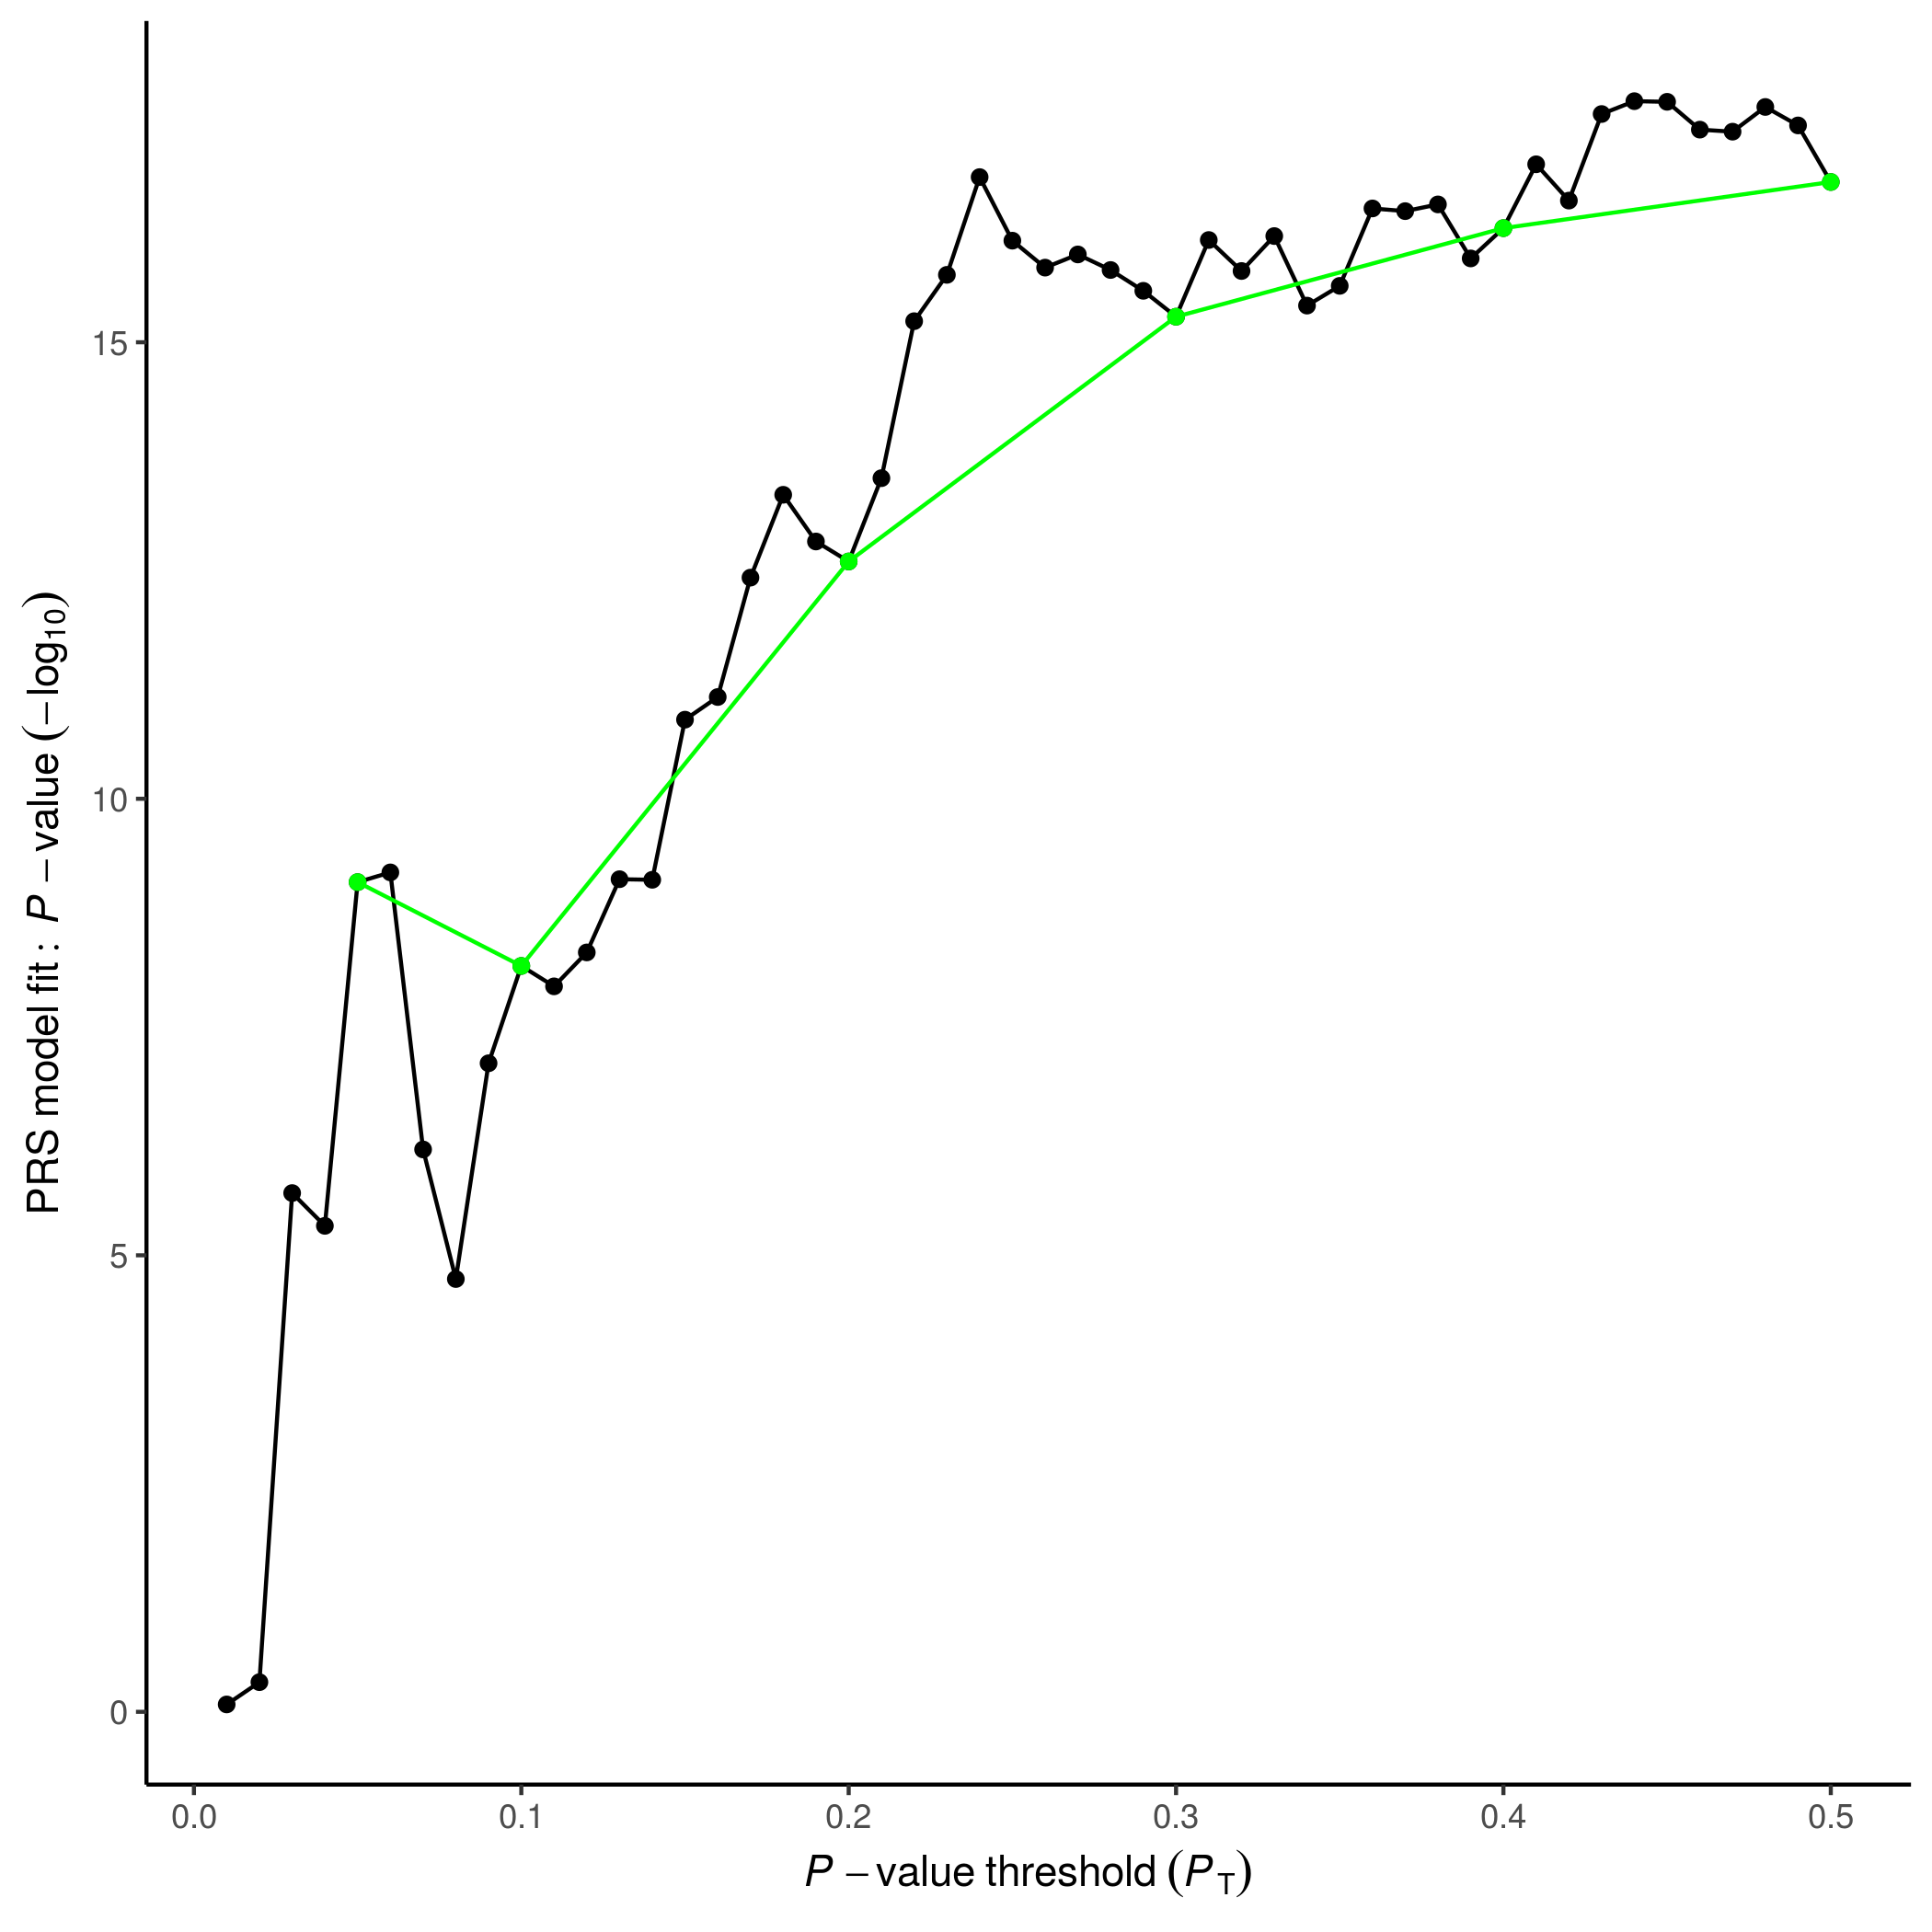
\includegraphics[width=0.35\textwidth]{EXAMPLE_1_HIGH-RES_PLOT_2017-06-02.png}}\hspace{1in}
\subfloat[Barplot]{\label{EXAMPLE_1_BARPLOT_2017-06-02.png}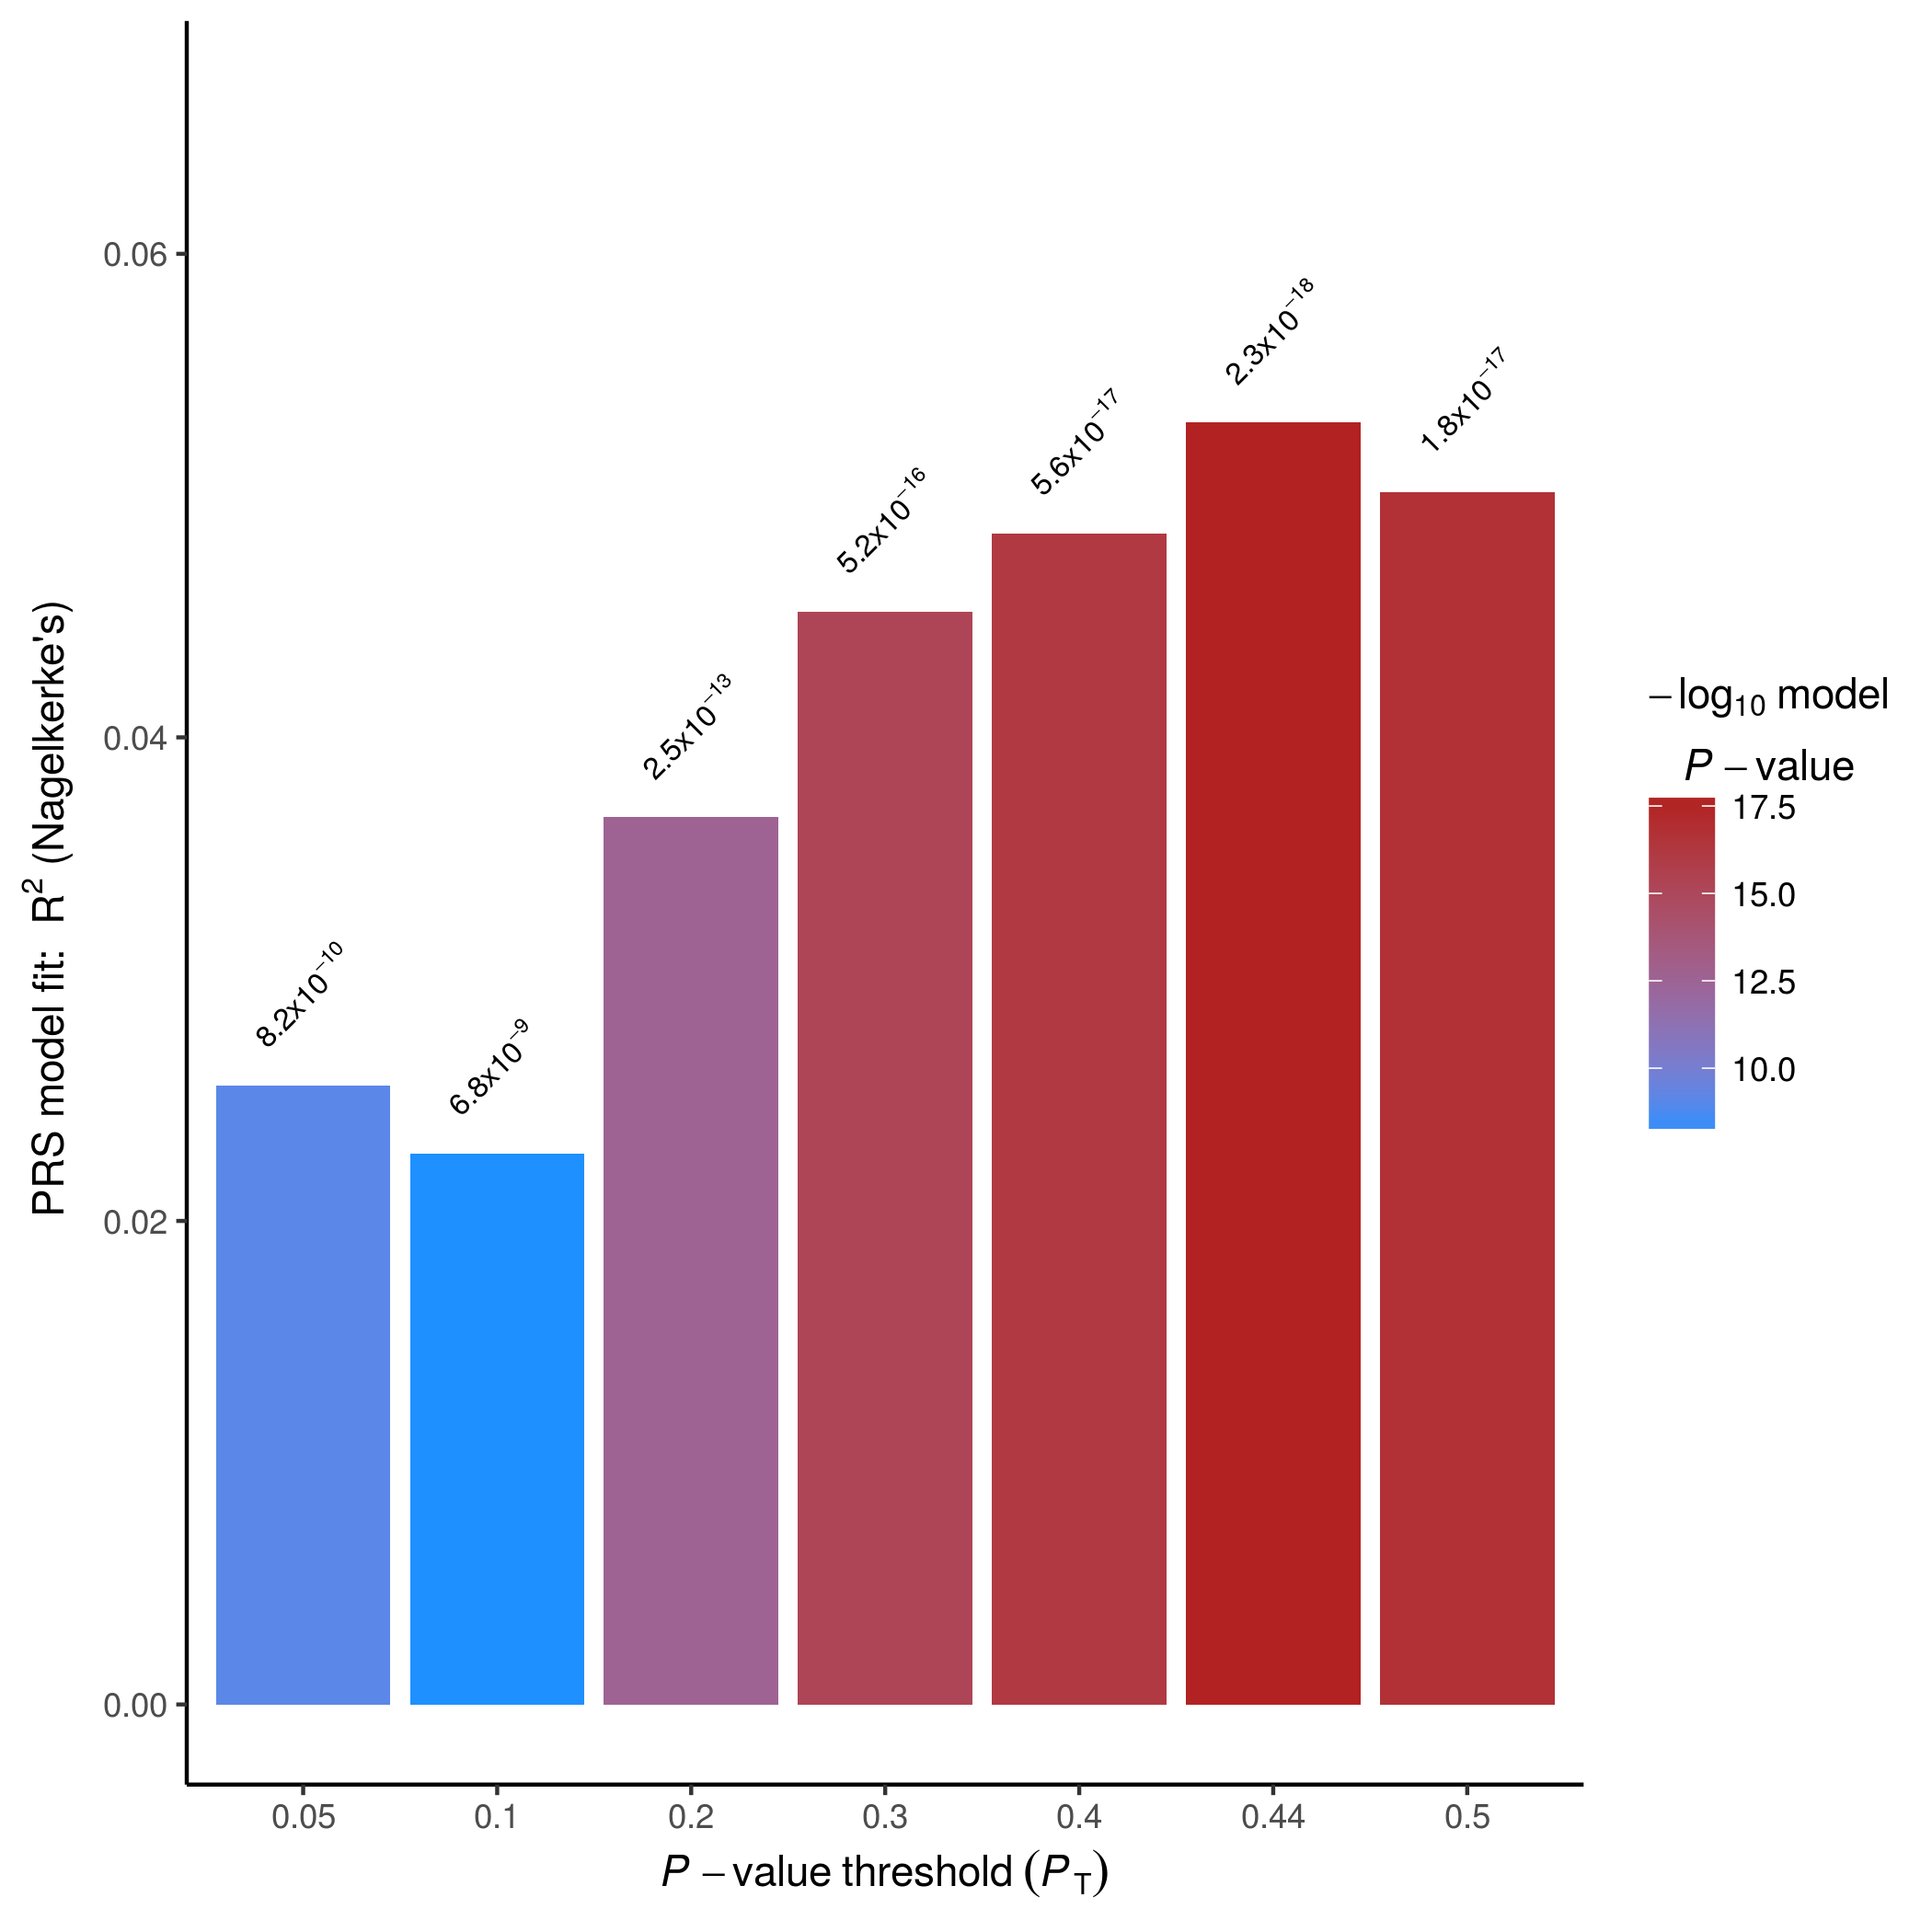
\includegraphics[width=0.35\textwidth]{EXAMPLE_1_BARPLOT_2017-06-02.png}}\\
\end{figure}

Figure \ref{PRSiceFigure} shows the two different outputs from this command. The second command line software which we will examine is \texttt{LDpred}: a Python based software package that adjusts GWAS summary statistics for the effects of linkage disequilibrium (LD). In order to calculate polygenic scores from this software package, we need to execute three commands, and one way to do this simultaneously is via a shell script:\\


\begin{listing}[H]
\caption{A Script for LDPred}\vspace{-0.1in}
\begin{minted}[mathescape, linenos, numbersep=5pt, gobble=0, frame=lines, framesep=2mm]{bash}
echo ''Now Running: coord_genotypes''
python ldpred/coord_genotypes.py \ 
--gf=test_data/LDpred_data_p0.001_test_0 \
--ssf=test_data/LDpred_data_p0.001_ss_0.txt --N=100 --out=bogus.hdf5
echo ''Now Running LDpred.py''
python ldpred/LDpred.py --coord=bogus.hdf5 --ld_radius=1 \
--PS=0.3 --N=100 --out=ldpredoutput
echo ''Running the validate.py''
python ldpred/validate.py \
--vgf=test_data/LDpred_cc_data_p0.001_train_0 \
--rf=ldpredoutput --out=pgsoutputs
\end{minted}
\end{listing}
\section{Conclusion} 

While we have introduced the command line, we have only begun to breach the surface of what it makes possible. There are a whole range of more advanced topics from both within a *nix-like operating system perspective (such as networking commands or process control and scheduling) as well as those concerning genomics and bioinformatics (such as SAMTools which provides a range of tools for manipulating read alignments or PLINK,  a free, open-source whole genome association analysis toolset). For this reason, we provide a reading list below to allow you to further explore the opportunities which the command line makes available.

\section{Further Reading}


\noindent
Chadwick, R. (2017), `Linux Tutorial', \url{http://ryanstutorials.net/}.\\

\noindent
Florea, L. (2017), `Command Line Tools for Genomic Data Science', Coursera Module: \url{https://www.coursera.org/learn/genomic-tools/home/welcome}.\\

\noindent
Kerrisk, M. (2010), `The Linux Programming Interface: A Linux and UNIX System Programming Handbook', No Starch Press, 1st Edition, ISBN: 1593272200. \\

\noindent
Marsh, N. (2010), `Introduction to the Command Line', Second Edition, Second Revision, ISBN: 1450588301.\\

\noindent
Sobell, M. (1994), `A Practical Guide to the UNIX System Paperback`, Pearson, Third Edition,  ISBN: 0805375651.\\
\end{document}